\documentclass[tikz,border=8pt]{standalone}
\usepackage{tikz}
\usepackage{fontawesome5}
\usepackage{amsmath,amssymb}
\usetikzlibrary{arrows.meta,positioning,fit,backgrounds,calc,shadows,shapes.geometric}

% Color definitions
\definecolor{lavenderDark}{RGB}{15, 44, 89}
\definecolor{lavenderDeep}{RGB}{10, 28, 58}
\definecolor{lavenderMedium}{RGB}{29, 78, 158}
\definecolor{lavenderLight}{RGB}{240, 246, 255}
\definecolor{lavenderBorder}{RGB}{180, 205, 237}
\definecolor{lavenderAccent}{RGB}{2, 132, 199}
\definecolor{prismNavy}{RGB}{15, 44, 89}
\definecolor{prismBlue}{RGB}{29, 78, 158}
\definecolor{prismTeal}{RGB}{13, 148, 136}
\definecolor{prismMint}{RGB}{236, 253, 245}
\definecolor{prismGold}{RGB}{217, 119, 6}
\definecolor{prismDark}{RGB}{15, 23, 42}
\definecolor{prismLight}{RGB}{248, 250, 252}
\definecolor{cInput}{RGB}{241, 245, 249}
\definecolor{cStem}{RGB}{224, 242, 254}
\definecolor{cStage1}{RGB}{209, 250, 229}
\definecolor{cStage2}{RGB}{254, 243, 199}
\definecolor{cStage3}{RGB}{254, 226, 226}
\definecolor{cStage4}{RGB}{207, 250, 254}
\definecolor{cHead}{RGB}{219, 234, 254}
\definecolor{cOutput}{RGB}{255, 228, 230}
\definecolor{cDeliverable}{RGB}{204, 251, 241}
\definecolor{statusFail}{RGB}{220, 38, 38}

\begin{document}
% End-to-End System Flow for Blockchain Voting DApp
\begin{tikzpicture}[
    x=1cm, y=1cm,
    hdrbox/.style={
        rectangle, draw=lavenderDark!80, line width=0.85pt, fill=lavenderDark!14,
        rounded corners=3pt, inner sep=4pt, align=center,
        text width=3.80cm,
        font=\fontsize{8.2}{9.8}\selectfont\bfseries\color{lavenderDark}
    },
    stepbox/.style={
        rectangle, draw=black!70, line width=0.7pt, fill=white,
        rounded corners=3pt, inner sep=3.8pt, align=center,
        text width=3.80cm,
        font=\fontsize{7.2}{8.5}\selectfont
    },
    stagebox/.style={
        rectangle, draw=lavenderDark!40, dashed, rounded corners=5pt, line width=0.8pt,
        fill=lavenderLight!25, inner xsep=5pt, inner ysep=6pt
    },
    transarr/.style={
        -{Stealth[length=4.5pt, width=3.5pt]}, line width=1.1pt, draw=lavenderMedium
    }
]

    % Column 1: Voter & MetaMask Client
    \node[hdrbox, fill=cInput] (c1_hdr) at (0, 0) {\faUser\ \textbf{Voter \& MetaMask}};
    \node[stepbox, below=0.6cm of c1_hdr] (s1_1) {
        \textbf{Access Voting Portal}\\
        Open \texttt{voting.html} in browser
    };
    \node[stepbox, below=0.6cm of s1_1] (s1_2) {
        \textbf{Connect MetaMask}\\
        Approve account access \& provide public address $v$
    };
    \node[stepbox, below=0.6cm of s1_2] (s1_3) {
        \textbf{Select Candidate $c$}\\
        Choose desired ballot option \& click Vote
    };
    \node[stepbox, below=0.6cm of s1_3] (s1_4) {
        \textbf{Sign Transaction}\\
        Cryptographically sign $\text{vote}(c)$ with ECDSA private key
    };

    % Column 2: Web3.js Middleware & RPC
    \node[hdrbox, fill=cStem, right=0.9cm of c1_hdr] (c2_hdr) {\faCode\ \textbf{React \& Web3.js}};
    \node[stepbox, below=0.6cm of c2_hdr] (s2_1) {
        \textbf{Fetch Candidates}\\
        Query contract for certified candidate array
    };
    \node[stepbox, below=0.6cm of s2_1] (s2_2) {
        \textbf{Local Pre-Validation}\\
        Verify voter status via \texttt{voters[address]}
    };
    \node[stepbox, below=0.6cm of s2_2] (s2_3) {
        \textbf{Construct Payload}\\
        Encode ABI invocation \texttt{vote(candidateId)}
    };
    \node[stepbox, below=0.6cm of s2_3] (s2_4) {
        \textbf{Relay via JSON-RPC}\\
        Broadcast raw signed transaction to Ethereum node
    };

    % Column 3: Smart Contract (EVM)
    \node[hdrbox, fill=cStage2, right=0.9cm of c2_hdr] (c3_hdr) {\faFileContract\ \textbf{Smart Contract (EVM)}};
    \node[stepbox, below=0.6cm of c3_hdr] (s3_1) {
        \textbf{Registration Check}\\
        \texttt{require(registered[v])}\\
        \textit{Revert if unauthorized}
    };
    \node[stepbox, below=0.6cm of s3_1] (s3_2) {
        \textbf{Double-Voting Mitigation}\\
        \texttt{require(!voters[v].hasVoted)}\\
        \textit{Atomic check $\text{Accept}(v)$}
    };
    \node[stepbox, below=0.6cm of s3_2] (s3_3) {
        \textbf{State Mutation}\\
        \texttt{voters[v].hasVoted = true}\\
        \texttt{candidates[c].voteCount++}
    };
    \node[stepbox, below=0.6cm of s3_3] (s3_4) {
        \textbf{Emit Event}\\
        \texttt{emit VoteCast(v, c, block.timestamp)}
    };

    % Column 4: Blockchain Ledger & Consensus
    \node[hdrbox, fill=cDeliverable, right=0.9cm of c3_hdr] (c4_hdr) {\faCube\ \textbf{Consensus \& Ledger}};
    \node[stepbox, below=0.6cm of c4_hdr] (s4_1) {
        \textbf{Mempool Ingestion}\\
        Transaction queued in pending validator pool
    };
    \node[stepbox, below=0.6cm of s4_1] (s4_2) {
        \textbf{PoA Block Sealing}\\
        Block mined by designated validator node
    };
    \node[stepbox, below=0.6cm of s4_2] (s4_3) {
        \textbf{Cryptographic Hash Chaining}\\
        $H(B_i) = \text{SHA-256}(H(B_{i-1}) \parallel \dots)$
    };
    \node[stepbox, below=0.6cm of s4_3] (s4_4) {
        \textbf{Immutable Receipt}\\
        Tx confirmed; Event captured by Web3 dashboard
    };

    % Background Stage Boxes
    \begin{scope}[on background layer]
        \node[stagebox, fit=(c1_hdr)(s1_4)] (col1_box) {};
        \node[stagebox, fit=(c2_hdr)(s2_4)] (col2_box) {};
        \node[stagebox, fit=(c3_hdr)(s3_4)] (col3_box) {};
        \node[stagebox, fit=(c4_hdr)(s4_4)] (col4_box) {};
    \end{scope}

    % Transition arrows across columns
    \draw[transarr] (s1_1) -- (s2_1);
    \draw[transarr] (s1_2) -- (s2_2);
    \draw[transarr] (s1_3) -- (s2_3);
    \draw[transarr] (s1_4) -- (s2_4);
    \draw[transarr] (s2_4) -- (s3_1);
    \draw[transarr] (s3_1) -- (s3_2);
    \draw[transarr] (s3_2) -- (s3_3);
    \draw[transarr] (s3_3) -- (s3_4);
    \draw[transarr] (s3_4) -- (s4_1);
    \draw[transarr] (s4_1) -- (s4_2);
    \draw[transarr] (s4_2) -- (s4_3);
    \draw[transarr] (s4_3) -- (s4_4);

    % Event Feedback Arrow to React
    \draw[transarr, dashed, draw=prismTeal] (s4_4.south) -- ++(0,-0.4) -| (s2_4.south)
        node[pos=0.25, below, font=\fontsize{6.5}{7.5}\selectfont, text=prismNavy] {Web3 Event Notification \& Real-Time UI Tally Update};

\end{tikzpicture}
\end{document}
